\chapter{RISC x CISC}

\textsc{Definição} \textbf{Gap Semântico:} diferença entre as operações oferecidas por uma linguagem e as operações oferecidas pela arquitetura.

A cada vez que as linguagens de programação iam se modernizando, o gap semântico ia aumentando. Ele deu origem a diversas ineficiências na execução dos programas, tamanho excessivo de código binário e complexidade do compilador.

Afim de reduzir esses efeitos, foram projetadas arquiteturas contendo grande número de intruções, diversos modos de endereçamento e instruções complexas oriundas das linguagens de alto nível, surgindo assim as máquinas com conjuntos complexos de intruções, as CISC.

\section{CISC}
Com instruções mais complexas, o objetivo era simplificar o compilador e melhorar o desempenho. Como instruções de alto nível já são traduzidas para linguagem de máquina, por haver uma instrução correspondente, a tradução é mais simples. Porém, um conjunto grande e complexo de instruções traz problemas:
\begin{itemize}
  \item O controle do mecanismos do pipeline é complicado;

  \item O compilador deve agora, ao analisar o código, saber quais instruções de alto nível podem ser diretamente mapeadas para as instruções complexas de máquina, o que nem sempre é fácil;

  \item Muitos compiladores acabam por deixar de usar instruções complexas em suas traduções

  \item O tamanho em bits das instruções em CISC acaba sendo maior que as de RISC;

\end{itemize}

Por isso, o código obtidos de arquitetura CISC são geralmente grande, ainda que visem serem pequenos, rápidos e menores que RISC. Os projetistas advogam que, com instruções maiores e mais complexas, o tempo de execução é reduzido. Porém a unidade de controle de máquinas CISC deve ser mais complexa, ocupando mais espaço, acabando por \textbf{aumentar o tempo de execução de uma única instrução}.


\section{RISC}
Em outra corrente, a eliminação do gap semântico é proposta com arquiteturas mais simples, as RISC. Aqui as instruções são mais simples, permitindo que uma instrução acabe em um ciclo de clock. É dada ênfase em operações entre registradores.

Essas arquiteturas são justificadas com base em estudos dos anos 80 com linguagens de alto nível, identificando que as operações mais abundantes são atribuições (passagem de dados) e desvios. Observou-se também que as variáveis acessadas eram em geral simples e locais, referenciado em média 0.5 operandos em memória e 1.4 registradores por instrução. Por fim, identificou-se que as procedures tinham chamadas menores que 6 parâmetros, usando menos que 6 variáveis locais. Logo não eram necessárias muitas palavras para ativar procedures.

Com base nisso, era mais interessante prover uma arquitetura que atacasse esses padrões de código mais utilizados, o que combinava mais com RISC, do que com arquiteturas que abarcassem aspectos mais gerais, o que se encaixava em CISC.

Como RISC veio como uma contra-proposta a CISC, diversas definições acabaram sendo atribuídas a RISC. Diz-se que "qualquer computador depois de 1985" é RISC. Porém, existem alguns pontos em comum.

\subsubsection{Grande Conjunto de Registradores}
Um número grande de registradores de propósito geral, com uso de compilador para otimizar seu uso. Como o número de atribuições observadas nos estudos eram grandes, os uso de vários registradores otimizava a execução.

Era necessária definir uma estratégia para manter os operandos mais utilizados em registradores e reduzir os acessos à memória. Daí, temos duas estratégias:
\begin{itemize}
  \item \textbf{Por software:} análise do compilador para tentar alocar registradores às variáveis mais utilizadas durante um certo período;

  \item \textbf{Por hardware:} grande conjunto de registradores, permitindo que mais variáveis sejam postas na CPU.
\end{itemize}

Deste último, nasceu a \textbf{janela de registradores}. O conjunto grande de registradores reduz o acesso à memória, mas o projetista deve organizar o acesso de maneira eficiente.

Como a maioria das referências é a variáveis locais, a abordagem mais comum é armazenar essas variáveis em registradores, separando alguns para as variáveis globais.

Porém, variáveis locais são atreladas ao contexto de sua procedure. Na chamada de uma procedure-filha, as variáveis tem de ser salvas em memória para poderem ser utilizadas posteriormente. Ao terminar, teríamos que carregar as variáveis da procedure-pai novamente juntamente com os valores de retorno da filha.

Para resolver isso, as janelas de registradores, que são vários pequenos conjuntos destes, são utilizadas para cada procedure. Uma chamada a uma procedure-filha faz com que uma janela de registradores diferente seja utilizada ao invés de salvar tudo e memória e trabalhar com um conjunto novo. Com isso, procedures adjacentes podem possuir janelas sobrepostas, para facilitar a passagem de parâmetros. Em dado momento, somente uma janela de registradores é visível e endereçavel.

A janela é dividida em 3 regiões de tamanho fixo:
\begin{itemize}
  \item Registradores de Parâmetros
  \item Registradores Locais
  \item Registradores Temporários
\end{itemize}

\begin{figure}[ht]
  \centering
  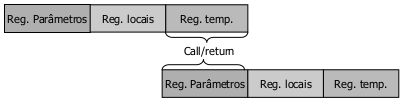
\includegraphics[width=.7\textwidth]{reg-window}
  \label{fig:reg-window}
  \caption{Esquema de uma janela de registradores. Perceba a sobreposição dos temporários e de parâmetros para permitir passagem de valores entre procedures}
\end{figure}

Como só existe um conjunto finito de janelas, somente os dados das procedures mais recentes são mantidos em registradores. Logo os dados de procedures antigas ficam em memória e a organização real do \textit{register file} é uma fila circular de janelas sobrepostas, como mostrado na \ref{fig:window-stack}.

\begin{figure}
  \centering
  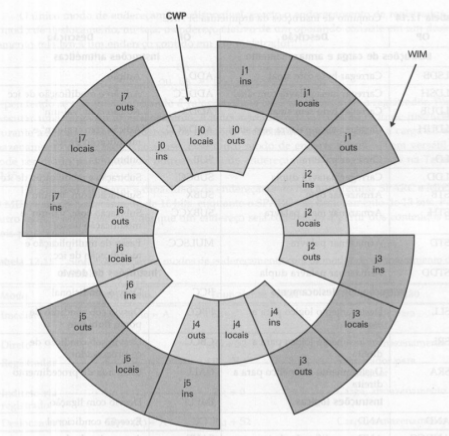
\includegraphics[width=0.66\textwidth]{reg-window-stack}
  \caption{Oito janelas de registradores formando uma pilha circular. Presente em arquiteturas SPARC}
  \label{fig:window-stack}
\end{figure}

\textsc{Variáveis Globais}\\
Se tratando de variáveis globais, inicialmente eram mantidas em memória, sugere-se mantê-las em um conjunto de \textbf{registradores globais} no processador. Estes registradores possuem número fixo e são acessíveis por todas as procedures.

\underline{Exemplo:} podemos dispor os registradores da seguinte forma
\begin{itemize}
  \item Registradores 0-7 contém variáveis globais
  \item Registradores 8-31: referem-se à janela corrente
\end{itemize}

\textsc{Otimizações pelo Compilador}\\
Como em programa escrito em linguagem de alto nível não faz referência a registradores, essa tarefa fica a cargo do compilador, que deve concentrar os acessos nos registradores, reduzindo \texttt{LOAD}s e \texttt{STORE}s.

Em geral, o compilador elege variáveis candidatas para residir em um registrador, chamadas \textbf{\textit{quantity}}, atribuindo-a à um registrador virtual. A idéia é mapear diversos registradores virtuais em um único registrador real, de modo que os virtuais não se sobreponham no tempo. Caso não haja número suficiente de registradores reais em um momento, o compilador recorre à memória.

Para aplicar esta técnica, são aplicados métodos de coloração de grafos. Primeiro o programa é analisado e um grafo de interferências de registradores é construído. O registradores virtuais são os nodos e as interdepêndencias são as arestas. Ao tentar colorir um grafo com $n$ cores, onde $n$ é o número registradores reais, mapeamos os nodos (virtuais) de mesma cor em único registrador real.

\begin{figure}
  \centering
  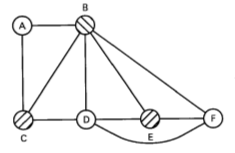
\includegraphics[width=0.6\textwidth]{reg-color-grafo}
  \label{fig:reg-color-grafo}
  \caption{Exemplo de coloração de grafo. Os conjuntos \{$A$, $D$\} e \{$B$, $C$, $E$\} são mapeados em registradores reais. $F$ é mapeado em memória.}
\end{figure}




\subsubsection{Conjunto Pequeno de Instruções}
O conjunto de instruções deve ser projetado de maneira que a grande maioria das \textbf{instruções sejam executada em um ciclo de máquina}, acelerando a execução de programas. A maioria das \textbf{instruções deve ser entre registradores, com operações de \texttt{LOAD} e \texttt{STORE} simples}, o que simplifica as unidades de controle.

A maioria das arquiteturas RISC oferece modos mais simples de endereçamento, geralmente menos que 5. Modos menos comuns de endereçamento, como o indireto e o indexado, podem ser sintetizados via software. Os mais comuns são:
\begin{itemize}
  \item Endereçamento de registradores
  \item ENdereçamento relativo ao PC
  \item Deslocamento
\end{itemize}

Não são usados modos de endereçamento que combinam load/store com operações aritméticas e somente um operando é endereçado a cada instrução. Logo, o formato de instruções são simples, o que permite:
\begin{itemize}
  \item O tamanho da instrução é fixo e alinhado por \textit{word}, com geralmente 4 bytes;

  \item A localização do código da operação é conhecida e de tamanho fixo. Ainda, a decodificação e buscas de operandos pode ser feita simultaneamente.
\end{itemize}

O compilador é uma parte fundamental para a obtenção de um bom código. Além disso, o desenvolvimento de chips RISC são mais rápidos, já que o número de instruções é simples e reduzido.




\subsubsection{Otimizações no pipeline de instruções}
Como arquiteturas RISC possuem instruções simples e regulares, acaba por ser mais fácil otimizar o \textit{hardware} e, consequentemente, no pipeline de instruções.





\section{RISC x CISC}
Observa-se que os projetos de arquitetura CISC vem empregando algumas características de RISC e vice-e-versa.

Como exemplos, as atuais arquiteturas do PowerPC, que é classificada como RISC, empregam implementações de CISC. O Pentium II, apesar de ser classificado como CISC, incorpora diversas características de RISC.

\begin{figure}[ht]
  \centering
  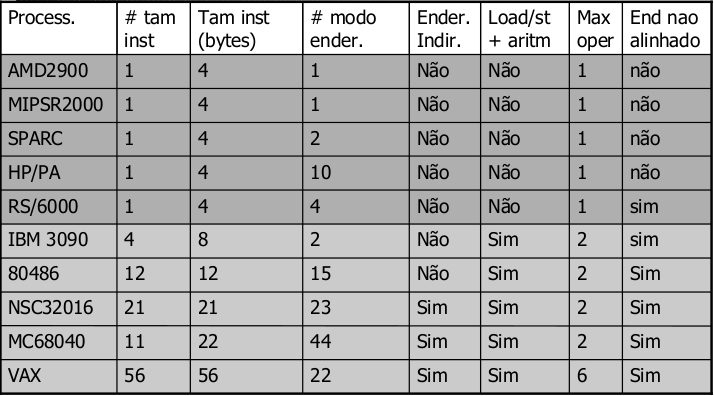
\includegraphics[width=0.75\textwidth]{risc-x-cisc}
  \label{fig:risc-x-cisc}
  \caption{Tabela comparativa de RISC (entradas escuras) X CISC (claras)}
\end{figure}
